\documentclass[tikz,border=10pt]{standalone}
\usepackage[T1]{fontenc}
\usepackage{amssymb}
\usetikzlibrary{positioning,arrows.meta,calc,fit,backgrounds}
\renewcommand{\familydefault}{\sfdefault}

% Okabe-Ito, matches the paper's oiblue/oiorange
\definecolor{cSeed}{RGB}{0,114,178}
\definecolor{cLint}{RGB}{86,180,233}
\definecolor{cSem}{RGB}{230,159,0}
\definecolor{cReal}{RGB}{0,158,115}
\definecolor{cDrop}{RGB}{213,94,0}
\definecolor{cBench}{RGB}{70,70,70}

\begin{document}
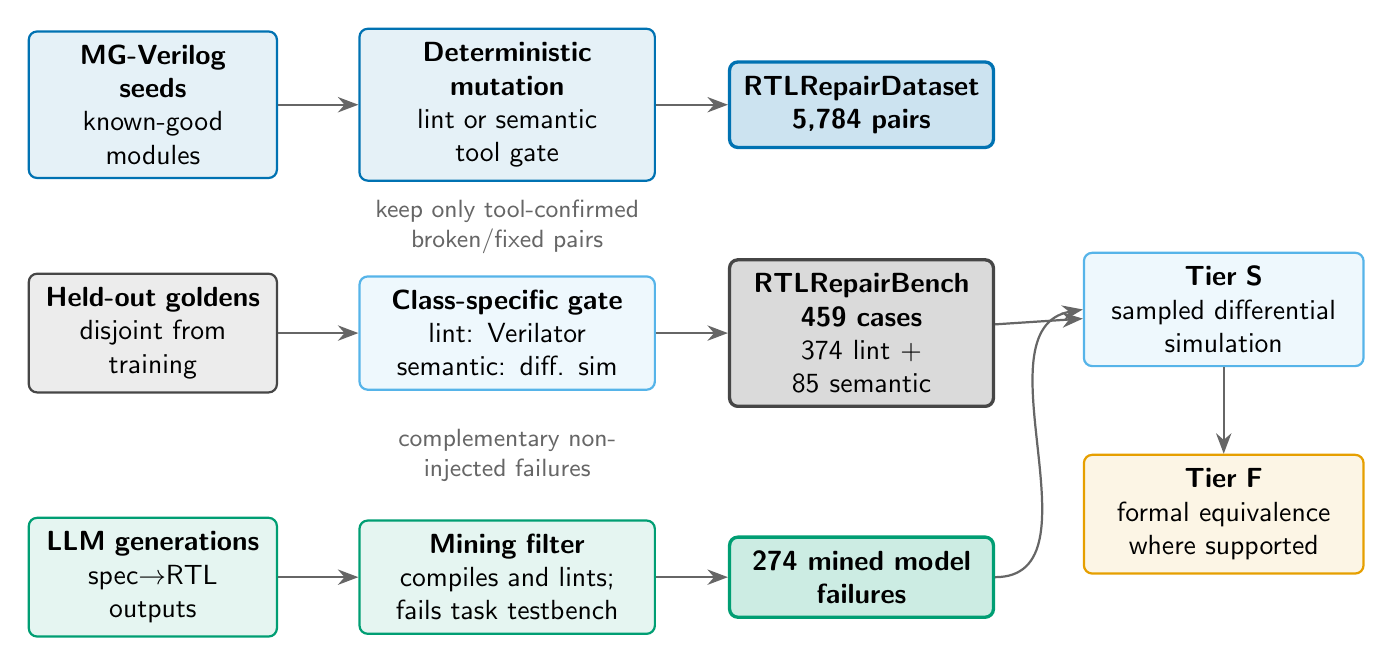
\begin{tikzpicture}[
  font=\normalsize,
  box/.style 2 args={rounded corners=3pt, draw=#1, fill=#1!10, thick,
    align=center, inner sep=5pt, text width=#2},
  result/.style={rounded corners=3pt, draw=#1, fill=#1!20, very thick,
    align=center, inner sep=5pt, font=\normalsize\bfseries},
  lbl/.style={font=\small, text=black!60, align=center},
  arr/.style={-{Stealth[length=2.6mm]}, thick, black!60},
]

% Training-resource track.
\node[box={cSeed}{2.8cm}] (trainseed) at (0,2.2)
  {\textbf{MG-Verilog seeds}\\ known-good modules};
\node[box={cSeed}{3.4cm}] (traingate) at (4.5,2.2)
  {\textbf{Deterministic mutation}\\ lint or semantic\\ tool gate};
\node[result=cSeed, text width=3.0cm] (trainout) at (9.0,2.2)
  {RTLRepairDataset\\ 5,784 pairs};

% Held-out benchmark track.
\node[box={cBench}{2.8cm}] (benchseed) at (0,-0.7)
  {\textbf{Held-out goldens}\\ disjoint from training};
\node[box={cLint}{3.4cm}] (benchgate) at (4.5,-0.7)
  {\textbf{Class-specific gate}\\ lint: Verilator\\ semantic: diff. sim};
\node[result=cBench, text width=3.0cm] (benchout) at (9.0,-0.7)
  {RTLRepairBench\\ 459 cases\\ \normalfont 374 lint + 85 semantic};

% Mined-failure track.
\node[box={cReal}{2.8cm}] (gen) at (0,-3.8)
  {\textbf{LLM generations}\\ spec$\to$RTL outputs};
\node[box={cReal}{3.4cm}] (mine) at (4.5,-3.8)
  {\textbf{Mining filter}\\ compiles and lints;\\ fails task testbench};
\node[result=cReal, text width=3.0cm] (realout) at (9.0,-3.8)
  {274 mined model\\ failures};

% Shared scoring contract.
\node[box={cLint}{3.2cm}] (tiers) at (13.6,-0.4)
  {\textbf{Tier S}\\ sampled differential\\ simulation};
\node[box={cSem}{3.2cm}] (tierf) at (13.6,-3.0)
  {\textbf{Tier F}\\ formal equivalence\\ where supported};

\draw[arr] (trainseed) -- (traingate);
\draw[arr] (traingate) -- (trainout);
\draw[arr] (benchseed) -- (benchgate);
\draw[arr] (benchgate) -- (benchout);
\draw[arr] (gen) -- (mine);
\draw[arr] (mine) -- (realout);
\draw[arr] (benchout) -- (tiers);
\draw[arr] (realout.east) to[out=0,in=190] (tiers.west);
\draw[arr] (tiers) -- (tierf);

\node[lbl, text width=3.4cm] at (4.5,0.65)
  {keep only tool-confirmed broken/fixed pairs};
\node[lbl, text width=3.4cm] at (4.5,-2.25)
  {complementary non-injected failures};

\end{tikzpicture}
\end{document}
